%!TEX root = ../dokumentation.tex

\chapter{Trainieren eines Klassifikationsmodells} \label{ch:crispDm_1}

% @Leo, sollen wir den Inhalt von Business Understanding als Einleitung für das Kapitel nehmen?

% \section{Business Understanding} \label{sec:businessUnderstanding}

In dem folgenden Abschnitt wird \ac{CRISP-DM} genutzt, um \ac{ML} Modelle zu trainieren, welche Texte einer der sechs politischen Parteien aus dem Deutschen Bundestag zuordnet. 

% TODO: Add missing sections

\ac{CRISP-DM} ist ein weitverbreitetes iteratives Modell, welches zur Strukturierung von Data-Mining Projekten genutzt wird \autocite{martinez-plumed_casp-dm_2017, chapman_crisp-dm_2000}. Das Modell besteht aus sechs Schritten: Business Understanding, Data Understanding, Data Preparation, Modeling, Evaluation und Deployment. 

\begin{figure}[H]
    \centering
    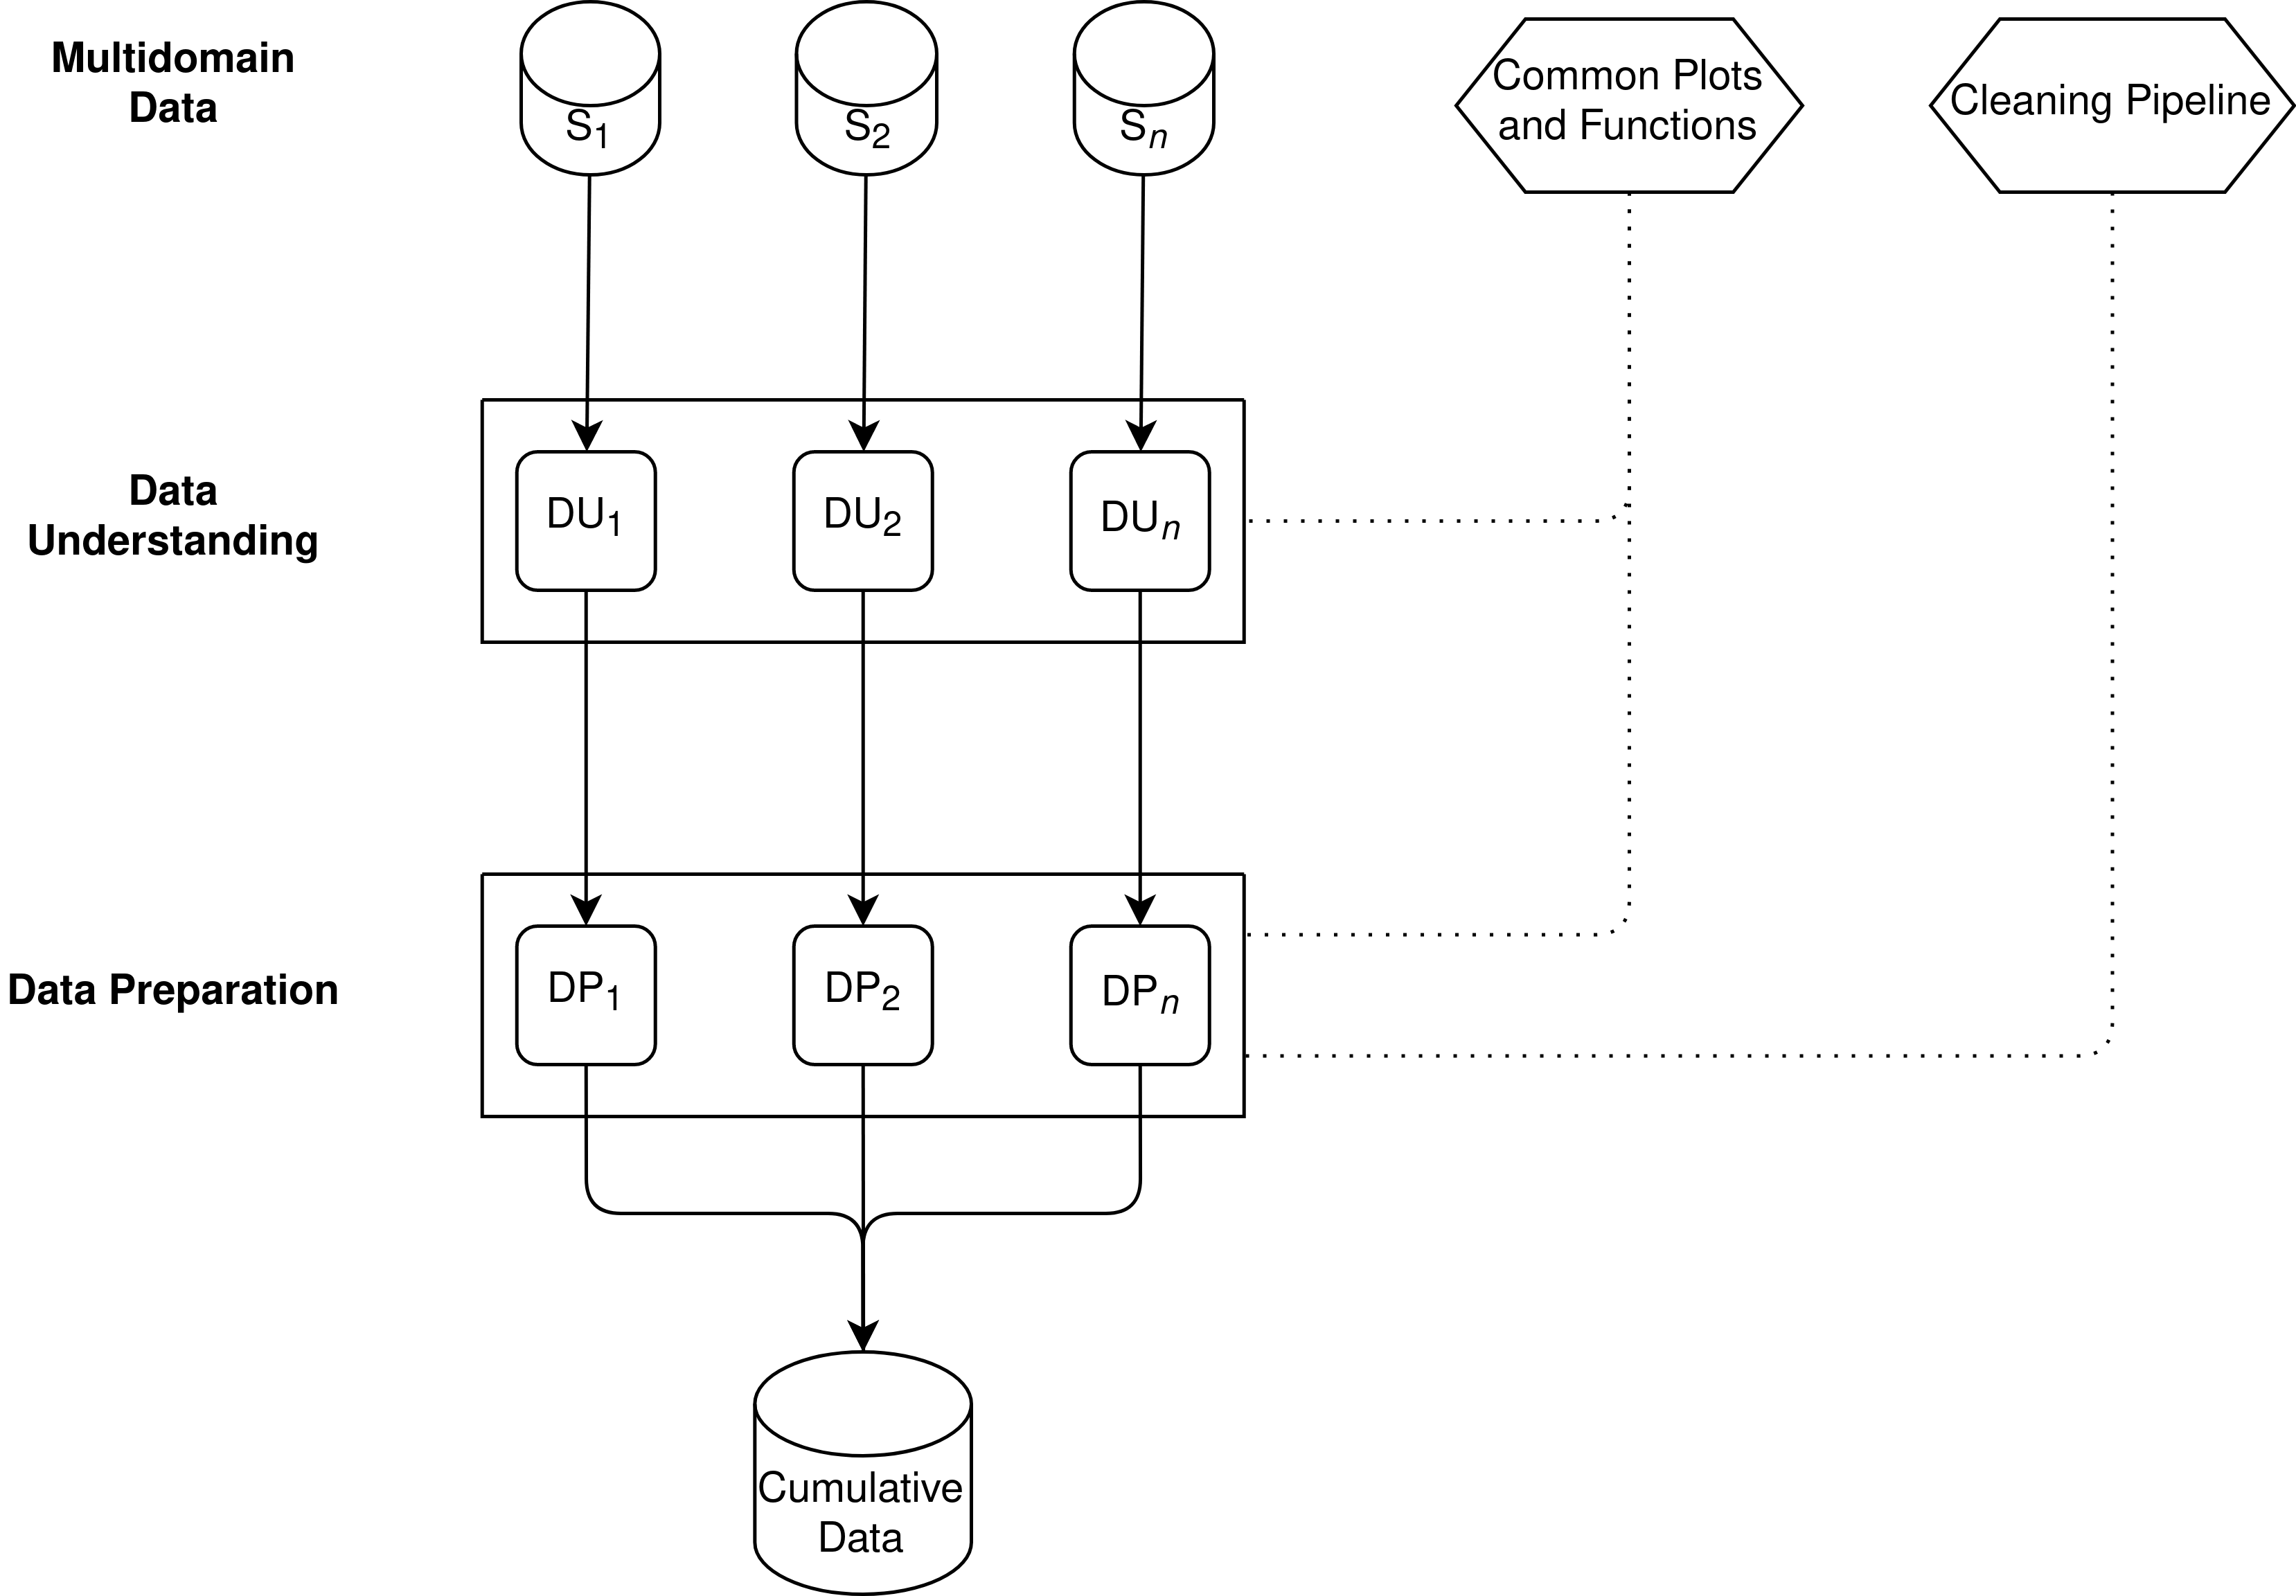
\includegraphics[width=0.8\textwidth]{data/images/data_flow_v2_1.png}
    \caption[Datenverarbeitungs-Pipeline]{Datenverarbeitungs-Pipeline (Data Understanding, Data Preparation und Zusammenführung der Daten)} \label{fig:dataFlow_1}
\end{figure}

% TODO: Add source for multidomain data

Multidomain Daten (z. B. Reden, Zeitungsartikel und Social Media Nachrichten) ermöglichen es, generalisierter \ac{ML} Modelle zu trainieren. Da die Daten stark voneinander abweichen, ist es notwendig, dass die unterschiedlichen Datenquellen im Prozess des Data Understandings und Data Preparation individuell verarbeitet werden. Nachdem jeder Datensatz einzeln analysiert und bereinigt wurde, werden die Daten für das Modeling zusammengeführt.

% \begin{figure}[H]
%     \centering
%     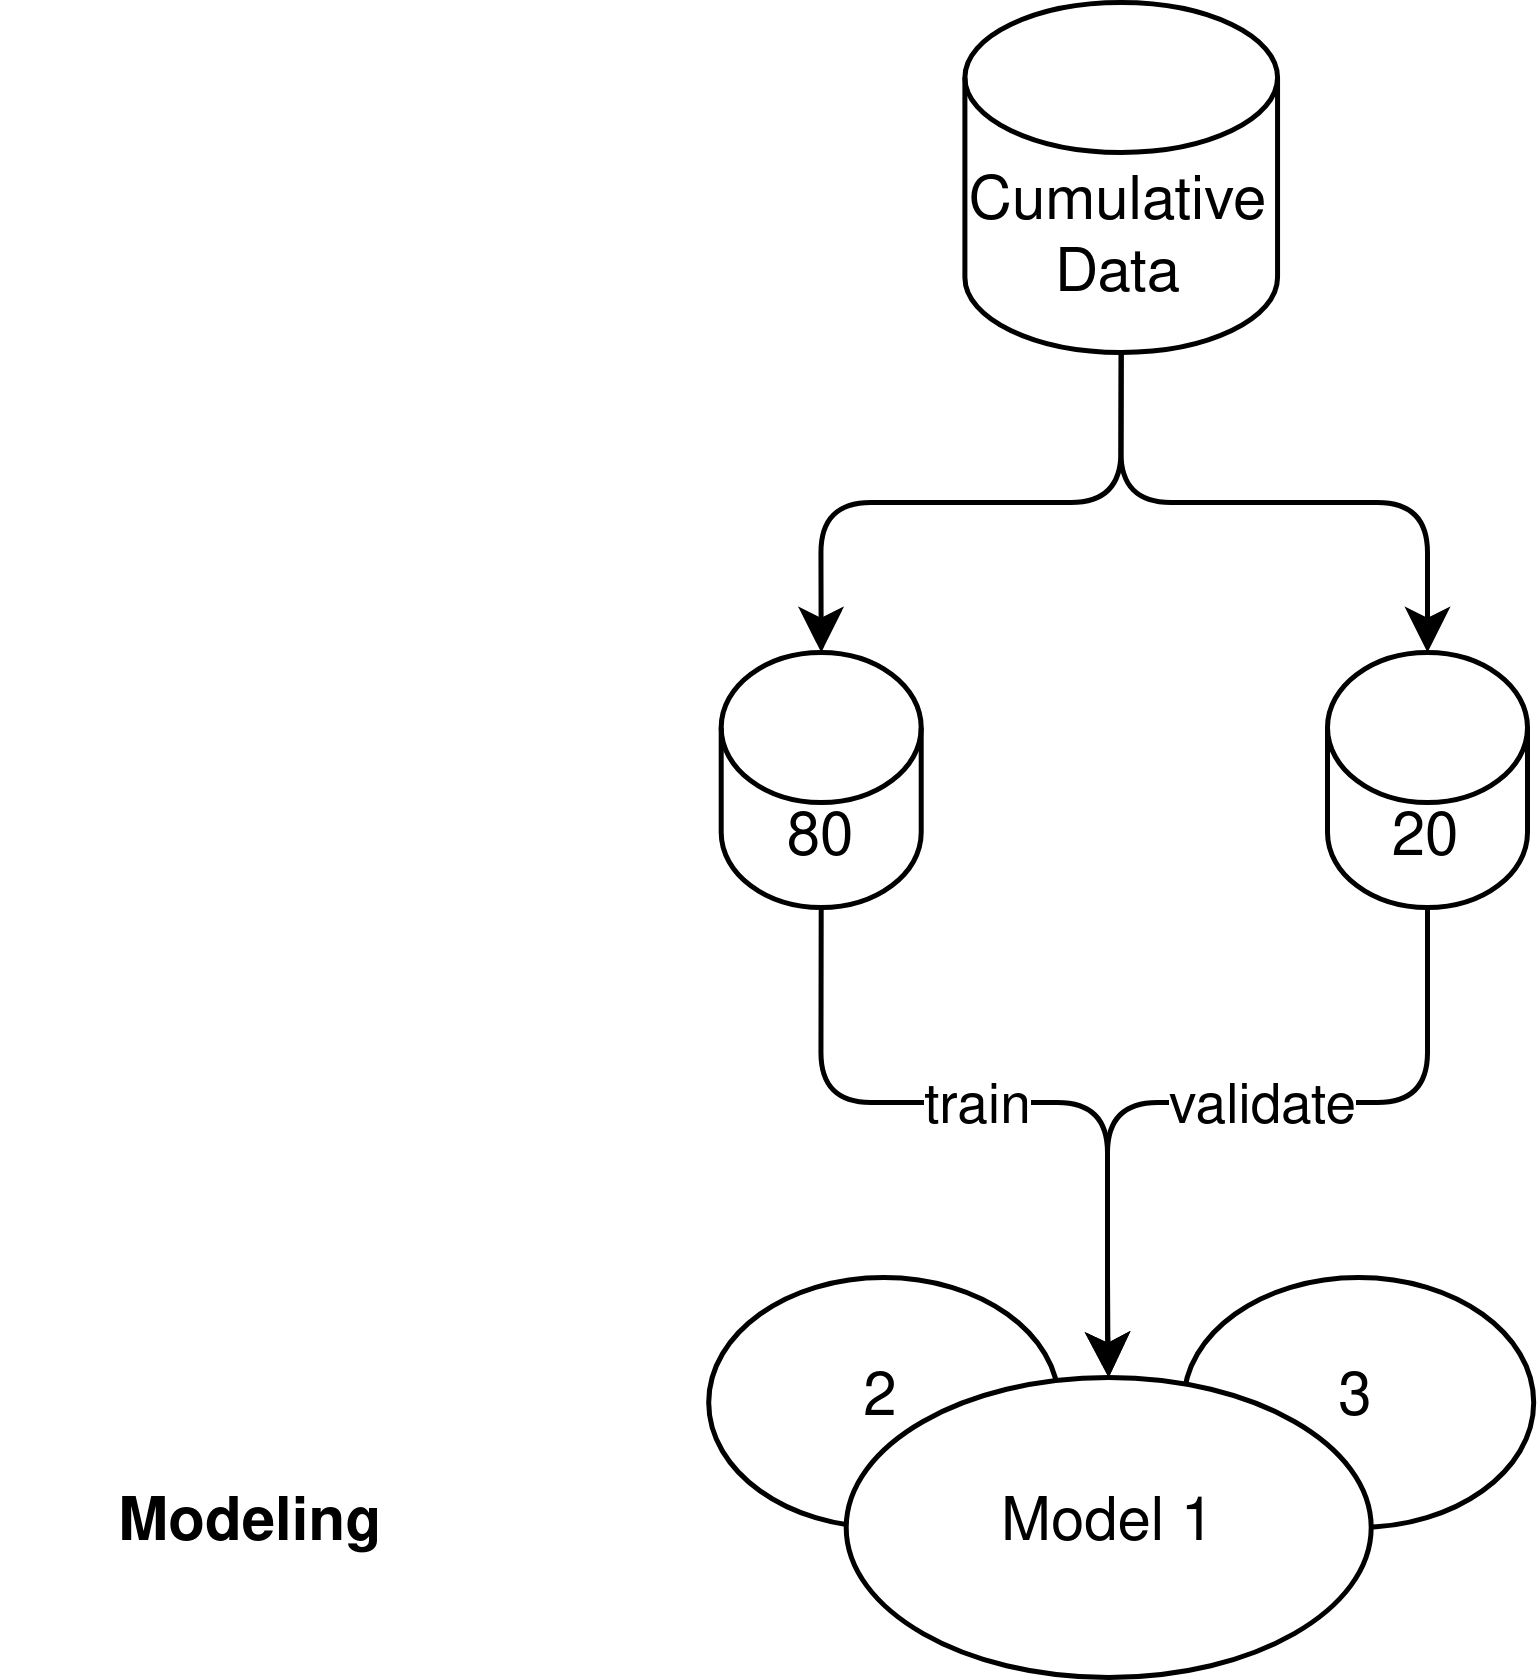
\includegraphics[width=0.4\textwidth]{data/images/data_flow_v2_2.png}
%     \caption[Training von Modellen]{Training von Modellen (Modeling)} \label{fig:dataFlow_2}
% \end{figure}

\section{Datensätze} \label{sec:dataUnderstanding}

% TODO: Update values

\begin{table}[H]
    \centering
    {\footnotesize
    \begin{tblr}{width=\textwidth, hlines, vlines} % , colspec={l{0.15\textwidth}XXXXXXl{0.15\textwidth}}
        \textbf{Datensätze} & \textbf{AfD} & \textbf{Die Grünen} & \textbf{SPD} & \textbf{CDU} & \textbf{Die Linke} & \textbf{FDP} & \textbf{Gesamt\-anzahl} \\ 

        Tweets & \num{187} & \num{187} & \num{187} & \num{187} & \num{187} & \num{187} & \num{1337} \\
        Wahlpro\-gramme & \num{187} & \num{187} & \num{187} & \num{187} & \num{187} & \num{187} & \num{1337} \\
        Reden & \num{187} & \num{187} & \num{187} & \num{187} & \num{187} & \num{187} & \num{1337} \\

        \textbf{Summe} & \textbf{\num{187}} & \textbf{\num{187}} & \textbf{\num{187}} & \textbf{\num{187}} & \textbf{\num{187}} & \textbf{\num{187}} & \textbf{\num{1337}} \\
    \end{tblr}
    }
    \caption{Übersicht über gelabelte Datensätze} \label{tab:overviewDatasets}
\end{table}

- Multidomain Texte/Quellen
- Anzahl an Elementen pro Partei
- Anzahl an Sätzen / Zeichen `count\_sentence`
- Word count

\subsection{Tweets}

Der Tweet-Datensatz von \textcite{saltzer_finding_2022} umfasst \num{876118} Tweets von \num{511} Politikern des Deutschen Bundestages. Die Bundestagsabgeordneten gruppieren sich in acht Parteien\footnote{Die Grünen, \ac{SPD}, Die Linke, \ac{AfD}, \ac{FDP}, \ac{CDU}, \ac{CSU} und Parteilose}. Die Tweets decken einen Zeitraum von Januar \num{2017} bis Dezember \num{2019} ab. Unter den Politikern befinden sich \num{161} Frauen und \num{350} Männer.

% TODO: Update image

\begin{figure}[H]
    \centering
    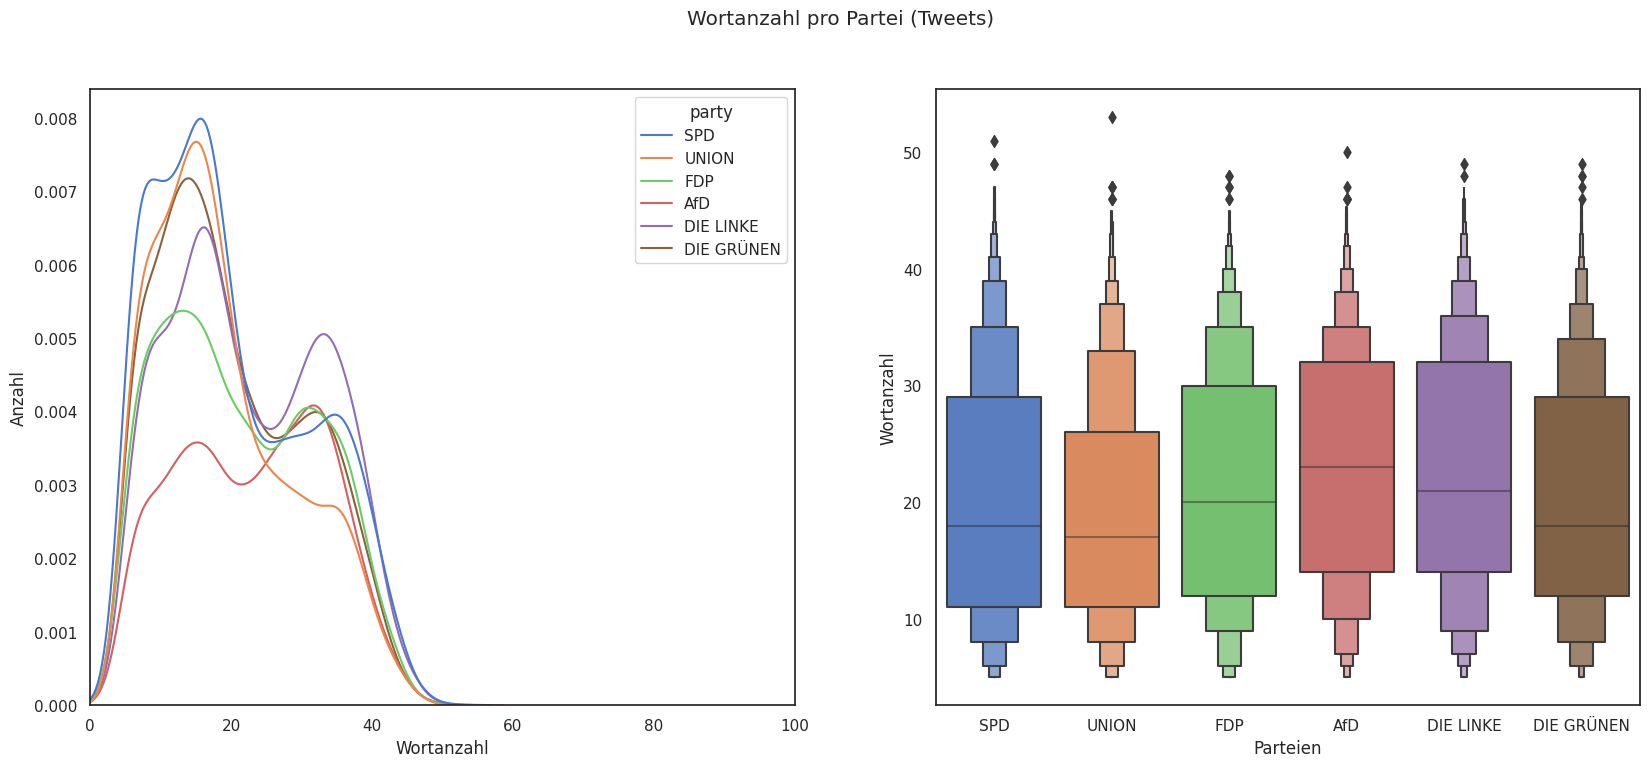
\includegraphics[width=0.9\textwidth]{data/images/tweets_word_count.png}
    \caption{Anzahl an Wörtern nach regelbasierten Bereinigen} \label{fig:wordCoundTweets}
\end{figure}

% TODO: Add reference

\autoref{fig:wordCoundTweets} zeigt die Verteilung der Wörteranzahl 

\section{Data Preparation} \label{sec:dataPreparation}

\subsection{Feature Engineering} \label{subsec:featureEngineering}

\subsubsection{Gewichtete Wörter}

- Bag of Words 
- Term Frequency - Inverse Document Frequency 
    - Berechnen der Frequency Parteiabhänig

\subsubsection{Word Embeddings}

Lorem Ipsum

\subsubsection{Sentiment}

Eine Limitation von den herkömmlichen \ac{ML} Modellen ist die Klassifikation von Polysemie \autocite[48\psq]{kowsari_text_2019}. 

% TODO: Find source

Ein Ansatz, um diese Limitation zu mindern, ist es, den Sentiment eines Textes zu berechnen. Ziel dieser Technik ist es nicht nur festzustellen, ob sich ein Politiker zum Beispiel zur \ac{AfD} äußert oder nicht, sondern ebenfalls, ob seine Äußerungen positiv, neutral oder negativ sind.

% TODO: Add timeline for ML Models

Die einfachste Methode um den Sentiment von deutschen Texten zu ermitteln sind Sentiment Wörterbücher wie \textit{SentiWS}, \textit{BAWL-R} und \textit{GermanPolarityClues} \autocite[1627\psq]{guhr_training_2020}. CNN, SVM, Bi-LSTM, ...

Die bisherigen regelbasierten Ansätze, als auch die \ac{ML} Modelle wie \acp{SVM}, \acp{CNN} und \acp{LSTM} erreichen lediglich einen F1 Scores von bis zu \num{74.9}. Alternativ zu diesen Ansätzen stellen \textcite{guhr_training_2020} ein \ac{BERT}-basiertes \ac{ML} Modell bereit. Dieses wurde mittels der folgenden Datensätze trainiert: \textit{PotTS}, \textit{SB10k}, \textit{GermEval-2017}, \textit{Scare}, \textit{Filmstarts}, \textit{holidaycheck}, \textit{leipzig-wikipedia} und \textit{Emotions}. Das Modell erreicht einen F1-Score von \num{0.9636} und ist somit den vorherigen Modellen deutlich überlegen \autocite[1631]{guhr_training_2020}.

\subsubsection{Gendern}

- Verhältnis Wörter/Gendersterne oder True/False
- Check mit RegEx ob gegendert wird und setze variable

\subsubsection{Dokumenttyp}

- Tweet, Speech, ...

\subsection{Cleaning Pipeline} \label{subsec:cleaningPipeline}

Stopwörter, Links, Symbole, Gendern und weitere Unregelmäßigkeiten (Rauschen, zu Englisch \textit{Noise}) können die Performance von \ac{ML} Modellen stark beeinflussen \autocite[4]{kowsari_text_2019}. Daher ist es notwendig Texte mittels regelbasierten Verfahren, als auch mit \ac{ML} Modellen zu bereinigen. 

% TODO: Insert image of cleaning pipeline

\begin{figure}[H]
    \centering
    \missingfigure{Cleaning Pipeline}
    \caption{Cleaning Pipeline} \label{fig:cleaningPipeline}
\end{figure}

\subsubsection{Regelbasierte Verfahren}

Im ersten Schritt der Bereinigung werden regelbasierte Verfahren genutzt, um Emojis, \acp{URL}, Verlinkungen von Nutzern, einzelne Buchstaben entfernt. Außerdem werden Zahlen mittels deren Text-äquivalent ausgetauscht. Schlussendlich werden alle Großbuchstaben zu Kleinbuchstaben konvertiert. 

- RegEx
    - Lower Case
    - Text in Kleinbuchstaben konvertieren
    - (Gendern entfernen)
    - (Nummern, Symbole und Zeichen)
    - Filter Personen
    - Filter Hashtags
    - Leerzeichen am Anfang und Ende entfernen
    % \subsection{Gendern} \label{subsec:gendering}

- Schwierigkeiten beim Verarbeiten von Texten, in welchen gegendert wird

\begin{enumerate}
    \item 
\end{enumerate}

% TODO: Update tweet example

\begin{code}[H]
    \begin{minipage}{0.45\textwidth}
        \small
        Ehemalige @AfD-Vorsitzende \#Petry muss wegen Meineid vor Gericht. Kein Einzelfall: gegen circa \SI{10}{\percent} aller AfD-Abgeordneten bundesweit laufen oder liefen Strafverfahren. Kriminelle Asylbewerber? Fehlanzeige. Kriminelle AfD-Hetzer trifft den Nagel eher auf den Kopf <U+0001F602> \#AfD
    \end{minipage}\hfill
    \begin{minipage}{0.45\textwidth}
        \small
        ehemalige petry muss wegen meineid vor gericht kein einzelfall gegen circa zehn prozent aller afd abgeordneten bundesweit laufen oder liefen strafverfahren kriminelle asylbewerber fehlanzeige kriminelle afd hetzer trifft den nagel eher auf den kopf afd
    \end{minipage}\hfill
    \caption[Beispiel -- Regelbasierte Bereinigung]{Beispiel für regelbasierte Bereinigung eines Tweets von \textit{victorperli} (links befindet sich der Ausgangstext und rechts der Text nach der regelbasierten Bereinigung} \label{list:rulebasedCleaning}
\end{code}

Unterschiedliche Formen, Slang und Rechtschreibfehler stellen ein elementares Problem für \ac{NLP} dar.

\subsubsection{Stemming}

Lorem Ipsum

% TODO: Update tweet example

\begin{code}[H]
    \begin{minipage}{0.45\textwidth}
        \small
        ehemalige petry muss wegen meineid vor gericht kein einzelfall gegen circa zehn prozent aller afd abgeordneten bundesweit laufen oder liefen strafverfahren kriminelle asylbewerber fehlanzeige kriminelle afd hetzer trifft den nagel eher auf den kopf afd
    \end{minipage}\hfill
    \begin{minipage}{0.45\textwidth}
        \small
        ehemalig petry muss wegen meineid vor gericht kein einzelfall gegen circa zehn prozent aller afd abgeordneter bundesweit laufen oder laufen strafverfahr kriminell asylbewerber fehlanzeig kriminell afd hetzer treffen der nagel eher auf der kopf afd
    \end{minipage}\hfill
    \caption[Beispiel -- Stemming]{Beispiel für Stemming eines Tweets von \textit{victorperli} (links befindet sich der Text nach der regelbasierten Bereinigung und rechts nach dem Stemming} \label{list:stemming}
\end{code}

\subsubsection{Stopwörter}

% TODO: Add more sources

Stopwörter sind Füllwörter, welche keine starke Relevanz für die Bedeutung eines Satzes haben \autocite[4]{kowsari_text_2019}. Das dadurch entstehende Rauschen kann unterdrückt werden, indem die Stopwörter gefiltert werden.

% TODO: Update tweet example

\begin{code}[H]
    \begin{minipage}{0.45\textwidth}
        \small
        ehemalig petry muss wegen meineid vor gericht kein einzelfall gegen circa zehn prozent aller afd abgeordneter bundesweit laufen oder laufen strafverfahr kriminell asylbewerber fehlanzeig kriminell afd hetzer treffen der nagel eher auf der kopf afd
    \end{minipage}\hfill
    \begin{minipage}{0.45\textwidth}
        \small
        ehemalig petry wegen meineid gericht einzelfall circa zehn prozent afd abgeordneter bundesweit laufen laufen strafverfahr kriminell asylbewerber fehlanzeig kriminell afd hetzer treffen nagel eher kopf afd
    \end{minipage}\hfill
    \caption[Beispiel -- Entfernen von Stopwörtern]{Beispiel für das Entfernen von Stopwörtern eines Tweets von \textit{victorperli} (links befindet sich der Text nach dem Stemming und rechts nach dem Entfernen von Stopwörtern} \label{list:stopwords}
\end{code}

\subsection{Filtering} \label{subsec:filtering}

\subsubsection{Tweets}

Um die Datenqualität der Tweets zu erhöhen, werden folgende Filterregeln angewandt:

\begin{itemize}
    \item \textbf{Duplikate}: Einige Tweets tauchen mehrfach mit einem abweichenden Erstellungsdatum auf.
    \item \textbf{Retweets}: Da die Intention und Meinung nicht zwangsweise von dem Politiker geteilt werden muss, werden Retweets entfernt.
    \item \textbf{Fehlende Einträge}: Manche Tweets beinhalten keine Nachricht.
    \item \textbf{Parteilos}: Parteilose stellen eine Gruppierung ohne identische politische Werte dar.
    \item \textbf{Wörteranzahl}: Sätzen mit zu wenigen Wörtern fehlt die grammatikalische Tiefe, welche \ac{NLP} erschwert (\texttt{stemm\_text >= 5}).
\end{itemize}

\section{Modeling} \label{sec:modeling}

- Datenquellen erst einzeln trainieren
- Datenquellen in verschiedenen Kombinationen trainieren
- Undersampling nach Partei 

% \subsection{Encoding}

% Für das Training von Klassifikationsmodellen wird zunächst die Partei (\texttt{party}) und das Geschlecht (\texttt{gender}) mittels Labelencoding encodiert.

\subsection{Baseline Models}

\subsection{FastText}

% TODO: Update and add plots for other datasets

\begin{figure}[H]
    \begin{subfigure}{.5\textwidth}
      \centering
      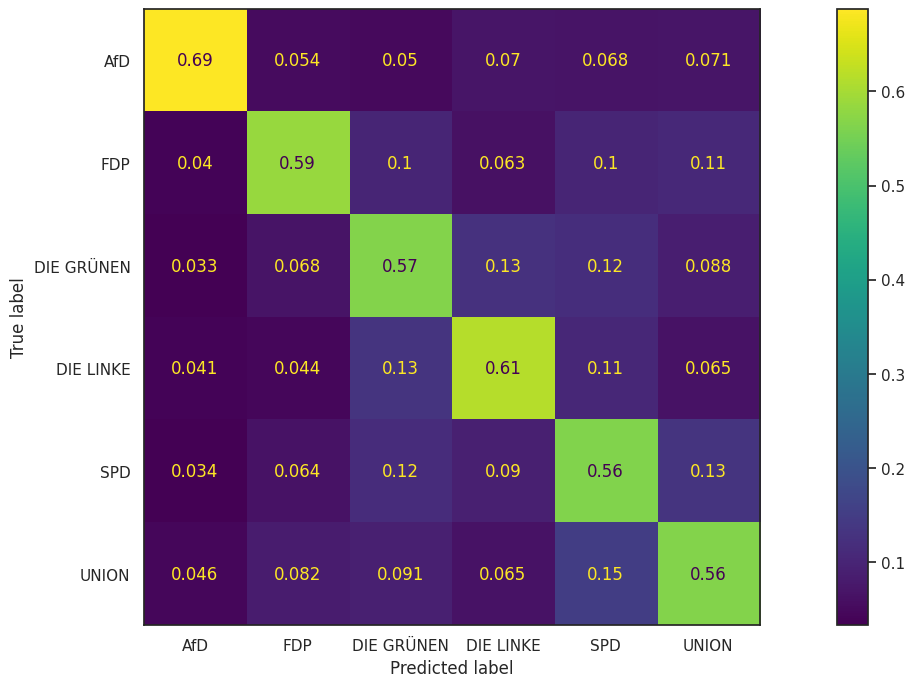
\includegraphics[width=0.9\linewidth]{data/images/fasttext_tweets_confusion.png}
      \caption{Tweets von \acs{MdB}} \label{sfig:confusionMatrixFastTextTweets}
    \end{subfigure}
    \begin{subfigure}{.5\textwidth}
      \centering
      \missingfigure{Wahlprogramme}
      \caption{Wahlprogramme} \label{sfig:confusionMatrixFastTextManifest}
    \end{subfigure}
    \begin{subfigure}{.5\textwidth}
      \centering
      \missingfigure{Reden}
      \caption{Reden im Deutschen Bundestag} \label{sfig:confusionMatrixFastTextSpeeches}
    \end{subfigure}
    \begin{subfigure}{.5\textwidth}
      \centering
      \missingfigure{Kombiniert}
      \caption{Kombinierten Datensatz} \label{sfig:confusionMatrixFastTextAll}
    \end{subfigure}
    \caption{Konfusion Matritzen für \texttt{fasttext}} \label{fig:confusionMatrixFastText}
\end{figure}

% TODO: Update scores

\begin{table}[H]
    \centering
    {\footnotesize
    \begin{tblr}{width=\textwidth, hlines, vlines}
        \textbf{Datensatz} & \textbf{Precision} & \textbf{Recall} & \textbf{\(F_1\) Score} \\ 

        Tweets & \num{0.59} & \num{0.59} & \num{0.59} \\
        Wahlpro\-gramme & \num{0} & \num{0} & \num{0} \\
        Reden & \num{0} & \num{0} & \num{0} \\

        \textbf{Kombiniert} & \textbf{\num{0}} & \textbf{\num{0}} & \textbf{\num{0}} \\
    \end{tblr}
    }
    \caption{Scores für Supervised Learning mittels \texttt{fasttext} (\texttt{weighted avg})} \label{tab:overviewScoresFastText}
\end{table}

\subsection{Limitationen}

\subsubsection{Feature Engineering}

% TODO: Add example for polysemy

Durch Methoden wie \ac{BoW} und \ac{TF-IDF} gehen syntaktische, als auch semantische Zusammenhänge verloren \autocite[48\psq]{kowsari_text_2019}. Dies führt dazu, dass Modelle wie \ac{SVM} und Random Forest ausschließlich die verwendeten Wörter und deren Anzahl in Betracht zieht, aber nicht die tiefere Bedeutung im Kontext des Satzes. Nach \textcite{kowsari_text_2019} versuchen Modelle wie Word2Vec, GloVe und \texttt{fasttext} zumindest syntaktische und semantische Zusammenhänge zu berücksichtigen, jedoch haben selbst diese Modelle Schwierigkeiten, Polysemie\footnote{Sätze mit mehreren Bedeutungen} zu klassifizieren.

\subsubsection{Sprache}

% TODO: Add sources and examples

Des Weiteren ergibt sich aus der Wahl der Datenquellen (Wahlprogramme, Reden und Tweets) eine Annahme/Voraussetzung/Bias geben über der verwendeten Sprache. Wahlprogramme, Reden und Tweets von Politikern weisen zwar parteispezifische Wörter auf, jedoch ist die semantische und syntaktische Komplexität der Sätze überdurchschnittlich hoch. Ebenfalls ist die Menge an Rechtschreibfehlern und verwendetem Slang geringer als bei anderen Textarten. Daraus folgt, dass die Performance der trainierten Modelle voraussichtlich signifikant schlechter ist, wenn Texte sprachlich (Semantisch und Syntaktisch) stark von den Trainingsdaten abweichen.

\subsubsection{Politische Nähe}

% TODO: Add sources and image
% TODO: Reason --> Politisches Viereck (links -- rechts, ...)

Parteien, welche ähnliche politische Ideale verfolgen, identische Themenschwerpunkte haben, lassen sich schlechter klassifizieren.

\section{Fazit} \label{sec:crispConclusion}

- Gender nicht kompatibel mit Lemmatizing und daher problematisch 
